\documentclass[12pt, a4paper]{article}
\usepackage[brazil]{babel}
\usepackage{amsmath}
\usepackage[utf8]{inputenc}
\usepackage[T1]{fontenc}
\usepackage{graphicx}
\usepackage{indentfirst}
\usepackage{hyperref}
\usepackage{url}
\urlstyle{same}
\setlength{\parindent}{1.25cm}

%Mudar orientação da página
\usepackage{lscape}

%Alterando a margem
\usepackage[margin=1in]{geometry}

%Não permitir frases estourarem a margem, principalmente urls
\sloppy

%Bibliografias
\usepackage{natbib}
\bibliographystyle{plain}

\title{Resultados do uso do algoritmo K-médias}
\author{Augusto Ribas$^1$, Bruno Nazário$^1$ e Doglas Sorgatto$^1$}
\date{$^1$Faculdade de Computação - Universidade Federal de Mato Grosso do Sul}

\begin{document}
\maketitle

\begin{abstract}
fhdfdjfdjfdjfhd
\end{abstract}
%
\section{Introdução}
jdhjdfhjdfhdhf


\subsection{Problema}
fjdhfjhfdjfd

\subsection{Objetivos}
Implementar o algoritmo K-médias sem utilizar as bibliotecas prontas disponíveis no Scikit-Learn \citep{scikit-learn} e aplicá-lo nos conjuntos de dados fornecidos pelo professor avaliando o desempenho


\section{Material e Métodos}
fhdfhdfdjfhdjfd

\subsection{Algoritmos de Agrupamento}
Clustering, ou Agrupamento,  é uma técnica de \textit{Data Mining} para fazer agrupamentos automáticos de dados segundo seu grau de semelhança. O critério de semelhança faz parte da definição do problema e, dependendo, do algoritmo conforme se lê em \citep{clustering}.

Normalmente o usuário do sistema deve escolher \textit{a priori} o número de grupos a serem detectados. Estes grupos são formados por equações que calculam a ``semelhança'' entre os dados através de funções de distância.

Os tipos de algoritmos de agrupamento de dados mais comuns são os: Particionais e os Hierárquicos. Os \emph{particionais} procuram criar grupos de semelhança.

De acordo com \citep{hierarquico}, ``Nos \emph{Hierárquico} o processo de identificação de grupos (clusters) é geralmente realimentado recursivamente, utilizando tanto objetos quanto grupos já identificados previamente como entrada para o processamento. Deste modo, constrói-se uma hierarquia de grupos de objetos, no estilo de uma árvore''.

\subsubsection{K-médias}
O algoritmo de agrupamento de dados K-Médias agrupa um conjunto de instâncias
em k partições, sendo k um número pré-estabelecido. O arranjo dos elementos é feito de maneira
que um elemento pertença a um cluster, cujo centro o elemento é mais próximo.
Dessa maneira, o algoritmo K-Médias consegue encontrar k partições disjuntas, buscando sempre
minimizar a variância intra-cluster e maximizar a variância inter-cluster. Como critérios de
convergência usuais, pode-se citar o número de iterações que o algoritmo executa e o número de
realocações de clusters.

\subsubsection{Arvore de Decisão}
fdfhdjfhdfdhj

\subsection{Procedimentos gerais}
fjdhfjdfdjfdjhf

\subsection{Conjuntos de dados}
Para este trabalho, 9 conjuntos de dados foram utilizados. Todos estes conjuntos são bi-dimensionais (isto é, têm 2 atributos), com o número de clusters variando de 2 a 10 (o primeiro conjunto tem 2 clusters, o segundo tem 3 clusters, e assim por diante). Todos estes conjuntos de dados apresentam uma partição de referência (grupo de cada um dos pontos), sendo perfeitamente balanceados (30 exemplos por grupo), como se observa na tabela \ref{conjDados}.
\begin{table}[!ht]
\centering
\caption{Características gerais dos conjuntos de dados}
\label{conjDados}
	\begin{tabular}{|l|c|c|}
	\hline
	Nome do conjunto & Número de instâncias & Número de grupos \\
	\hline
		artificial\_2.data & 60 & 2 \\
	\hline
		artificial\_3.data & 90 & 3 \\
	\hline
		artificial\_4.data & 120 & 4 \\
	\hline
		artificial\_5.data & 150 & 5 \\
	\hline
		artificial\_6.data & 180 & 6 \\
	\hline
		artificial\_7.data & 210 & 7 \\
	\hline
		artificial\_8.data & 240 & 8 \\
	\hline
		artificial\_9.data & 270 & 9 \\
	\hline
		artificial\_10.data & 300 & 10 \\
	\hline
	\end{tabular}
\end{table}

Cada um dos conjuntos de dados está disposto em um arquivo no formato CSV (\emph{``comma separated values''}). Em cada linha há um exemplo (instância) da base, no formato: $$Valor Atributo\_1, Valor Atributo\_2, Particao\_de\_Referencia$$ Sendo utilizado para o processamento apenas os dois primeiros atributos.

\section{Resultados e Discussão}

\begin{table}[!ht]
	\centering
	\caption{Comparação de eficiência - Menor SSE}	
	\label{tabMelhor}
	\begin{tabular}{|c|c|c|c|c|c|c|c|}
	\hline
	K & Seed & SSE & Convergir & Min & Max & Fora & Acurácia\\
	\hline
	2 & 2 & 1.17178486551 & 5 & 29 & 31 & 1 & 0.98333 \\
	\hline
	3 & 2 & 1.82592591238 & 5 & 30 & 30 & 0 & 1.00000 \\
	\hline
	4 & 0 & 2.40978786268 & 9 & 28 & 32 & 2 & 0.98333\\
	\hline
	5 & 6 & 2.47892858032 & 8 & 29 & 31 & 2 & 0.98666\\
	\hline
	6 & 10 & 3.38661981209 & 8 & 28 & 34 & 5 & 0.97222\\
	\hline
	7 & 4 & 3.64855687389 & 8 & 29 & 31 & & 0.98571\\
	\hline
	8 & 10 & 4.62062310715 & 5 & 25 & 35 & & 0.96250\\ %com seed 6 precisa de 18 para convergir com mesmo SSE e acuracia
	\hline
	9 & 16 & 4.6656708739 & 13 & 28 & 32 & & 0.98518\\
	\hline
	10 & 10 & 5.70866779082 & 11 & 28 & 32 & & 0.98333\\
	\hline
	\end{tabular}
\end{table}

\begin{table}[!ht]
	\centering
	\caption{Comparação de eficiência - Maior SSE}	
	\label{tabPior}
	\begin{tabular}{|c|c|c|c|c|c|c|c|}
	\hline
	K & Seed & SSE & Convergir & Min & Max & Fora & Acurácia\\
	\hline
	2 & 0 & 1.18583121013 & 4 & 27 & 33 & 3 & 0.95000 \\
	\hline
	3 & 8 & 4.18779991225 & 7 & 30 & 30 & 0 & 1.00000 \\
	\hline
	4 & 12 & 7.00024804537 & 4 & 28 & 32 & 2 & 0.98333\\
	\hline
	5 & 8 & 7.47642260367 & 50 & 0 & 61 & 60 & 0.60000\\
	\hline
	6 & 0 & 18.7881874706 & 50 & 0 & 123 & 120 & 0.33333\\
	\hline
	7 &  &  &  &  &  & &\\
	\hline
	8 &  &  &  &  &  & &\\
	\hline
	9 &  &  &  &  &  & &\\
	\hline
	10 &  &  &  &  &  & &\\
	\hline
	\end{tabular}
\end{table}


\begin{landscape}
\begin{figure}[!ht]
  \caption{Visão geral dos dados antes do agrupamento}
  \label{antes}
  \centering
    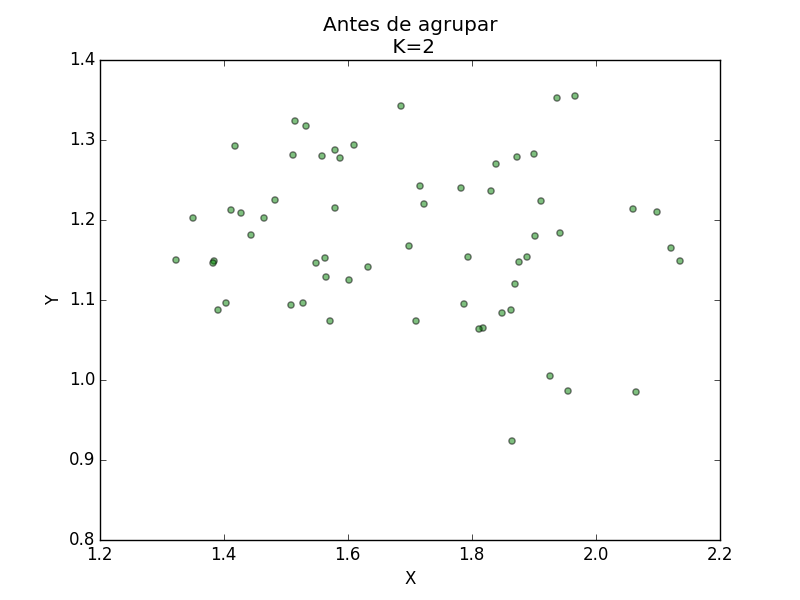
\includegraphics[width=0.4\textwidth]{antes_k2.png}
    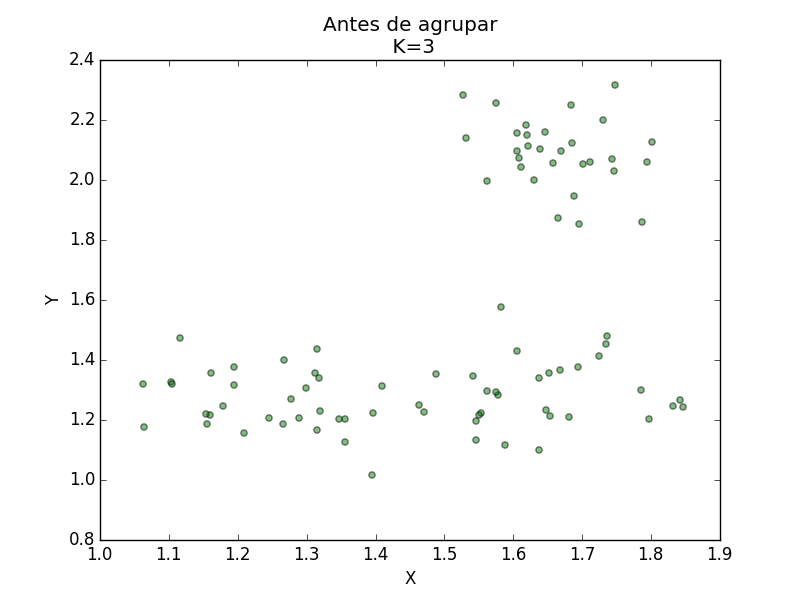
\includegraphics[width=0.4\textwidth]{antes_k3.png}
    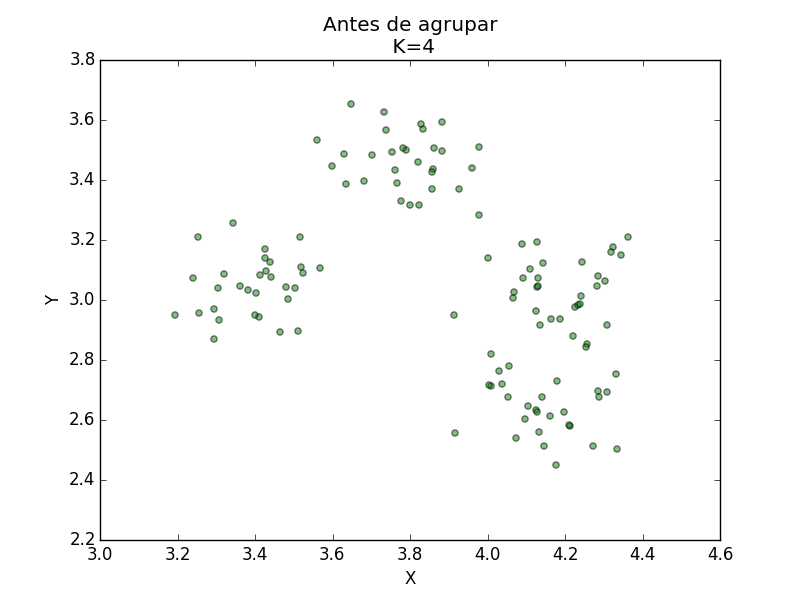
\includegraphics[width=0.4\textwidth]{antes_k4.png}
    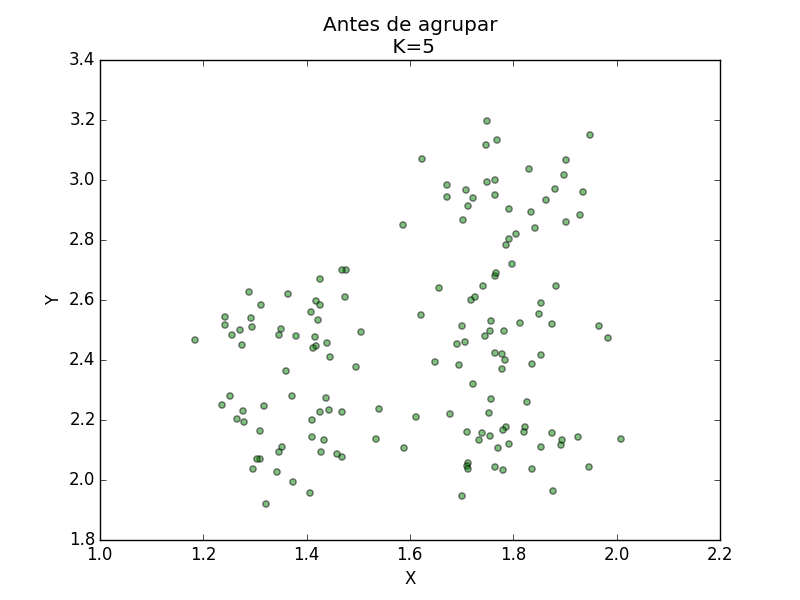
\includegraphics[width=0.4\textwidth]{antes_k5.png}
    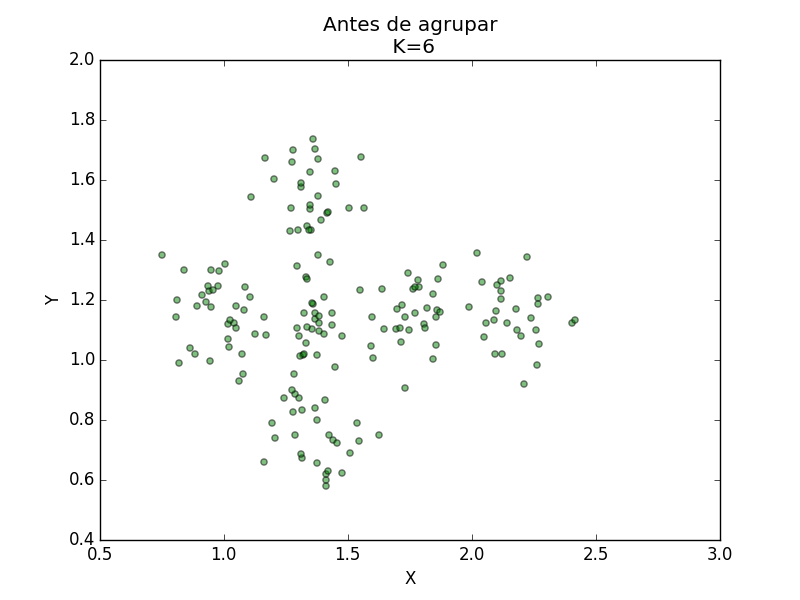
\includegraphics[width=0.4\textwidth]{antes_k6.png}
    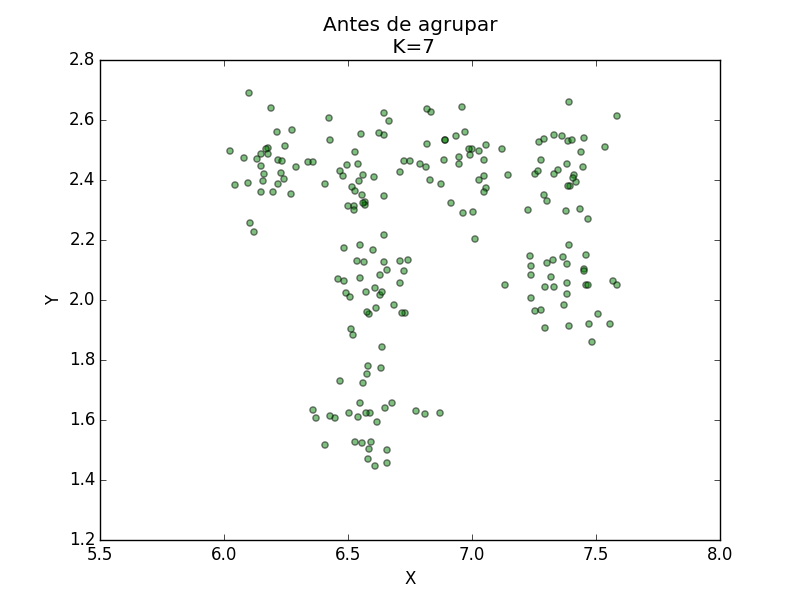
\includegraphics[width=0.4\textwidth]{antes_k7.png} 
    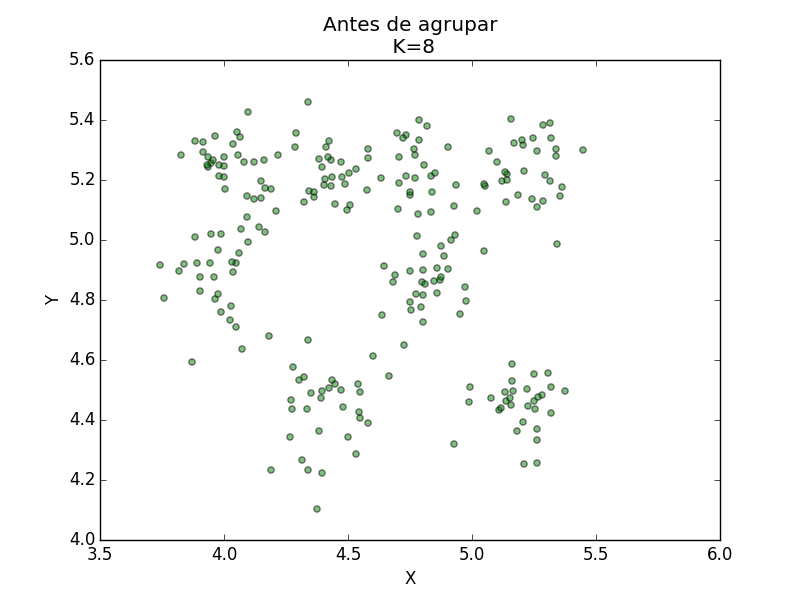
\includegraphics[width=0.4\textwidth]{antes_k8.png}    
    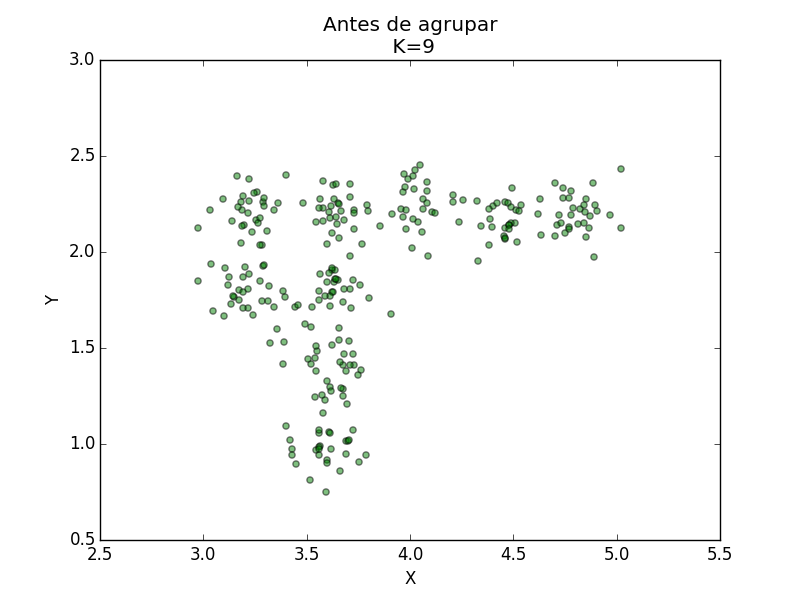
\includegraphics[width=0.4\textwidth]{antes_k9.png}
    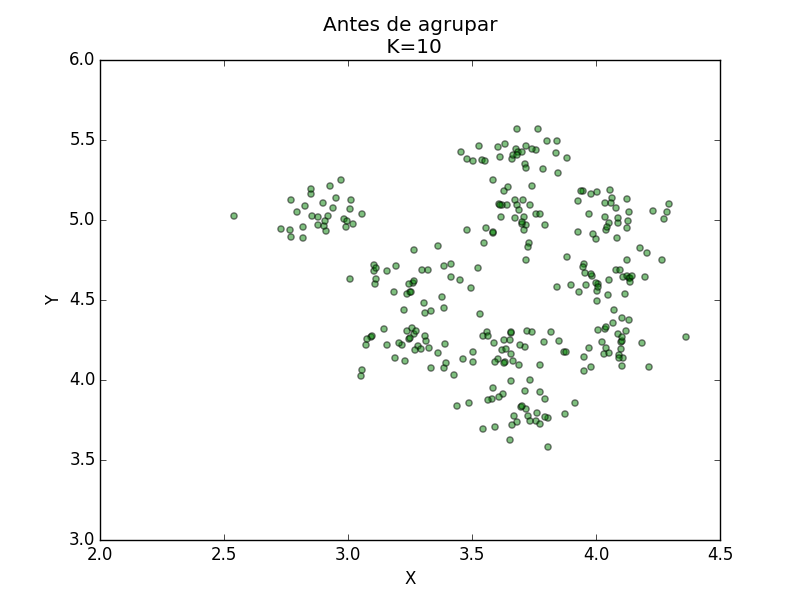
\includegraphics[width=0.4\textwidth]{antes_k10.png}          
\end{figure}
\end{landscape}

\begin{landscape}
\begin{figure}[!ht]
\label{erros}
  \caption{Evolução dos Somatórios de Erro Quadrático - SSE}
  \centering
    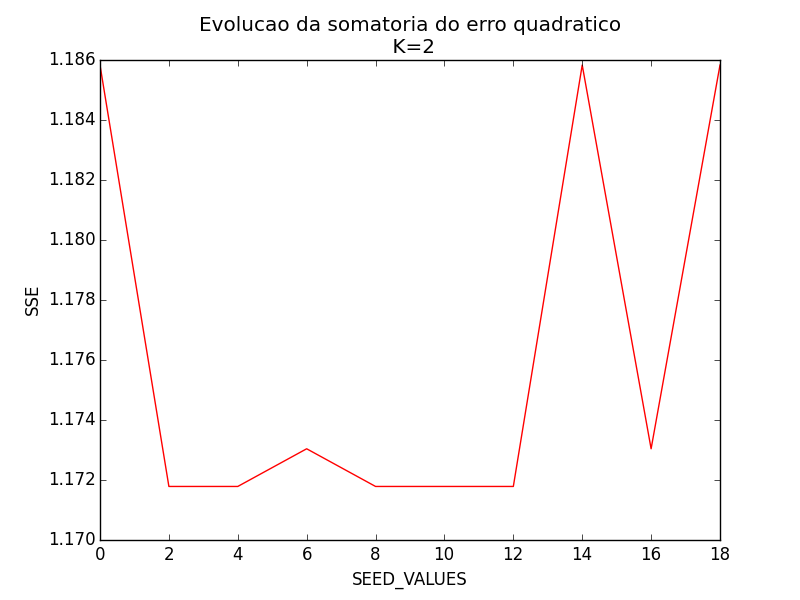
\includegraphics[width=0.4\textwidth]{erro_k2.png}
    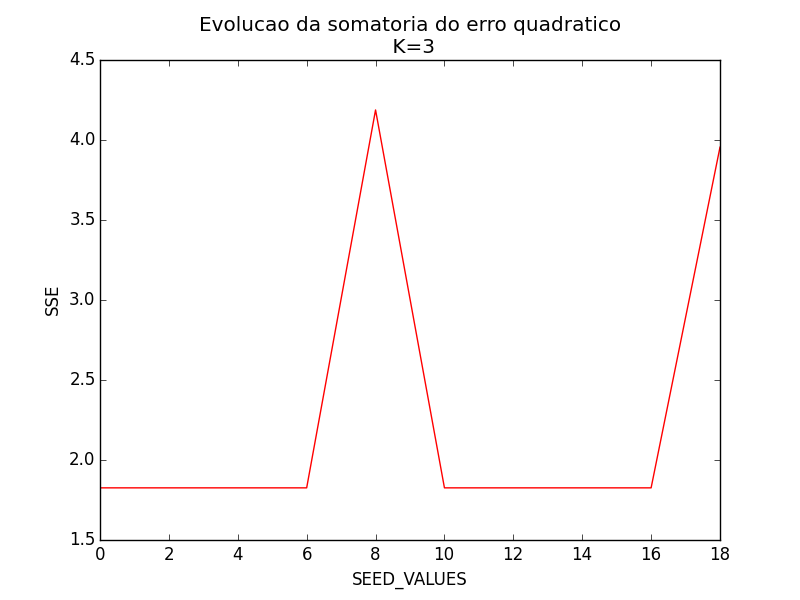
\includegraphics[width=0.4\textwidth]{erro_k3.png}
    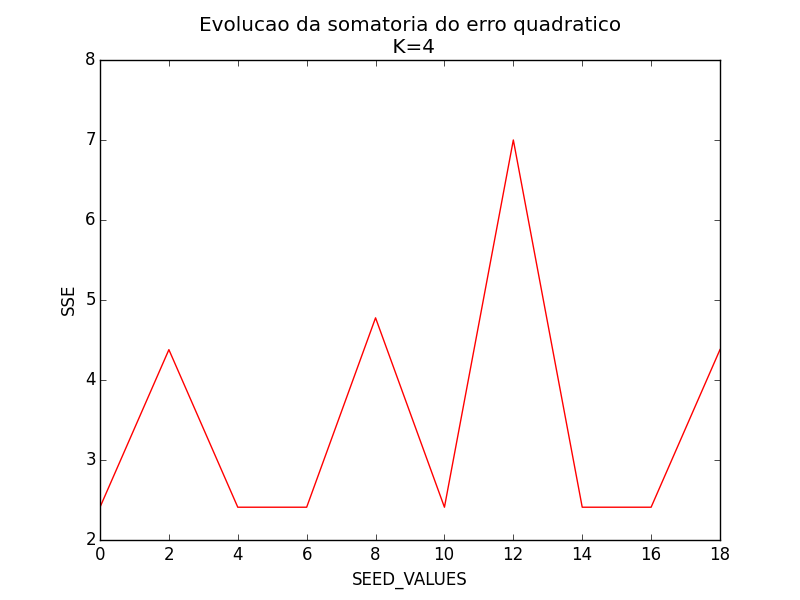
\includegraphics[width=0.4\textwidth]{erro_k4.png}
    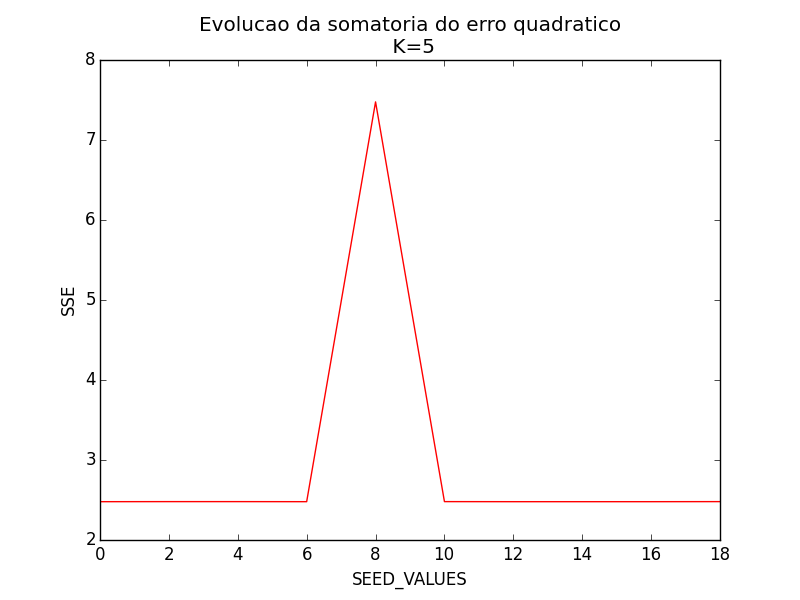
\includegraphics[width=0.4\textwidth]{erro_k5.png}
    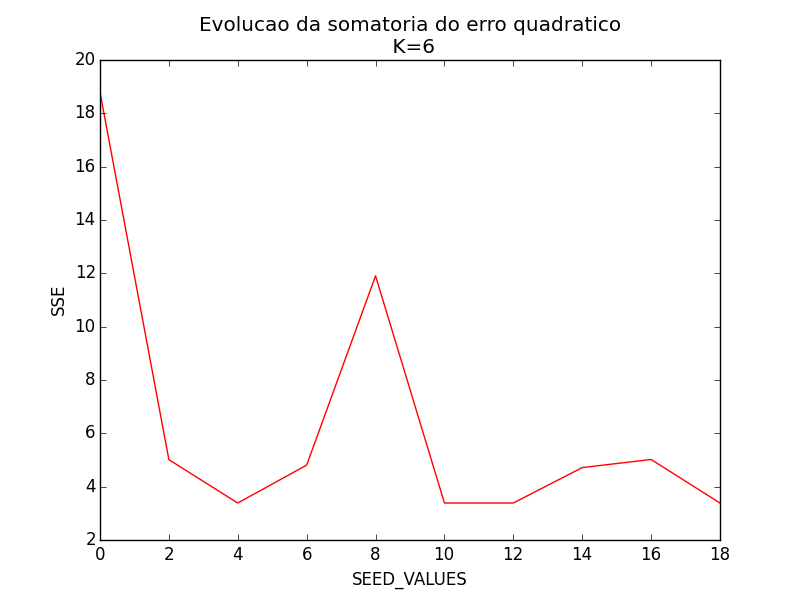
\includegraphics[width=0.4\textwidth]{erro_k6.png}
    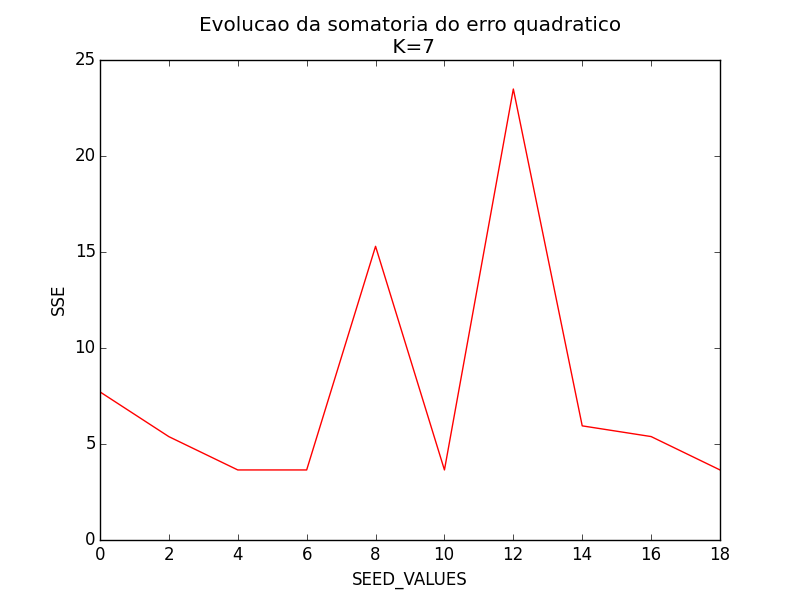
\includegraphics[width=0.4\textwidth]{erro_k7.png} 
    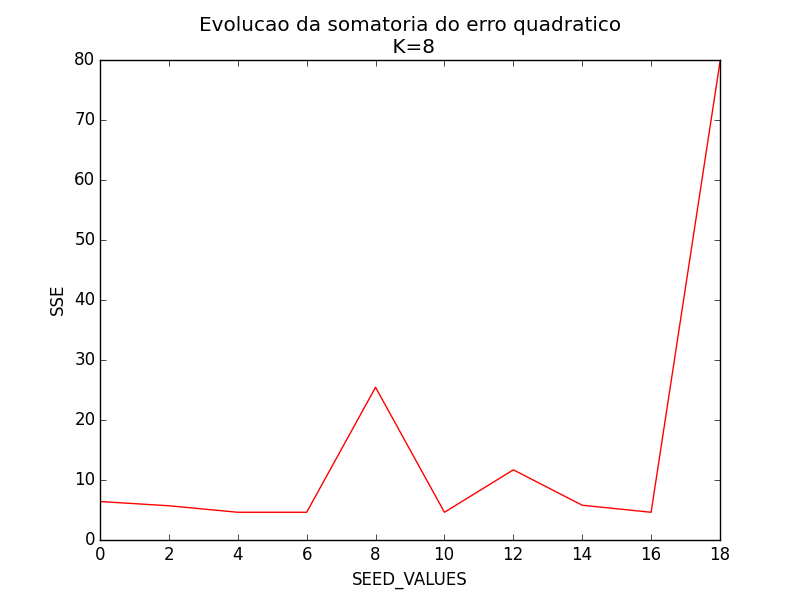
\includegraphics[width=0.4\textwidth]{erro_k8.png}    
    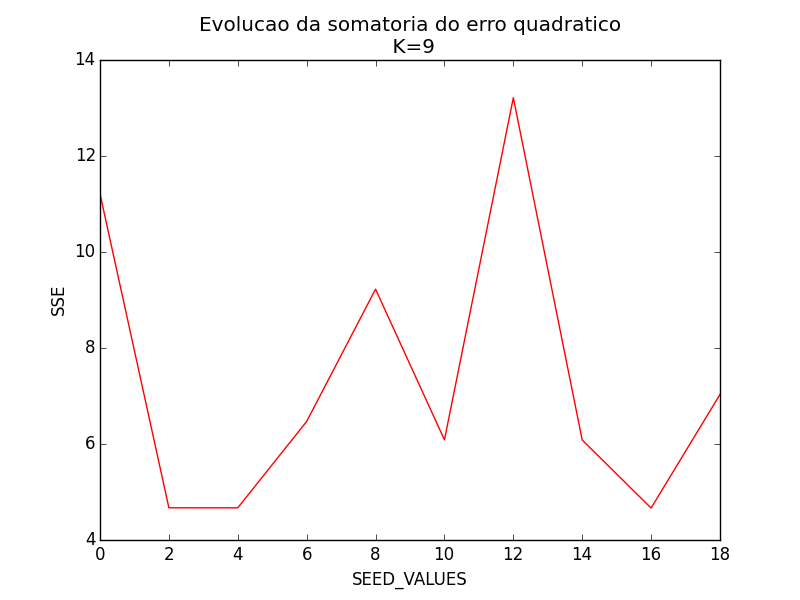
\includegraphics[width=0.4\textwidth]{erro_k9.png}
    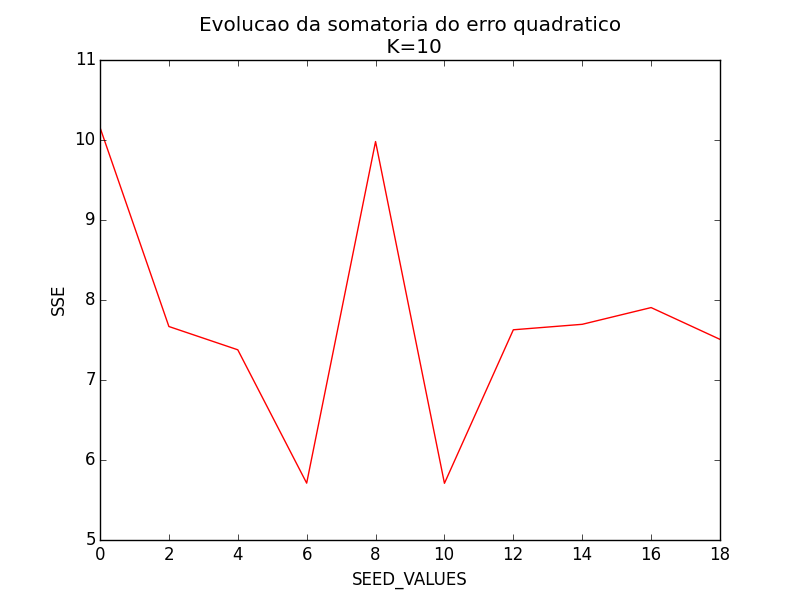
\includegraphics[width=0.4\textwidth]{erro_k10.png}
\end{figure}
\end{landscape}

\begin{landscape}
\begin{figure}[!ht]
\label{erros}
  \caption{Exemplo de evolução do processo de agrupamento para k = 5}
  \centering
    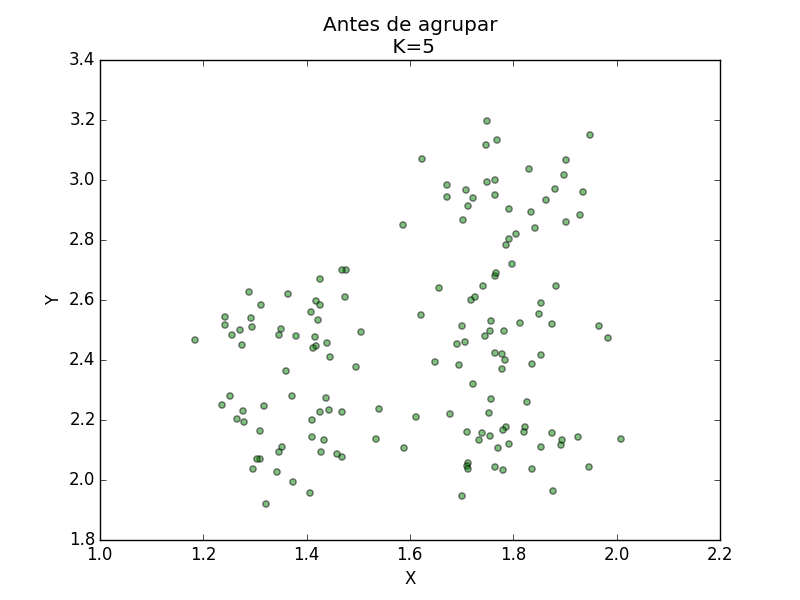
\includegraphics[width=0.4\textwidth]{antes_k5.png}
    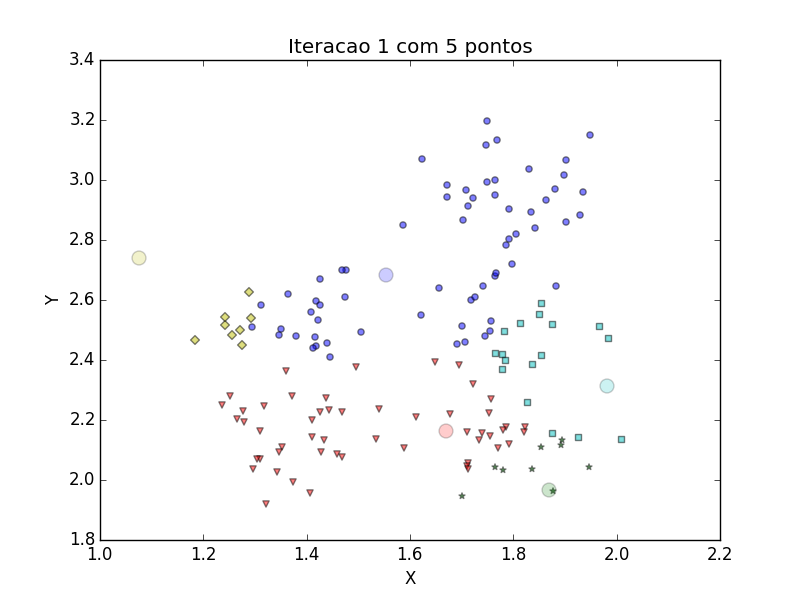
\includegraphics[width=0.4\textwidth]{depois_1.png}
    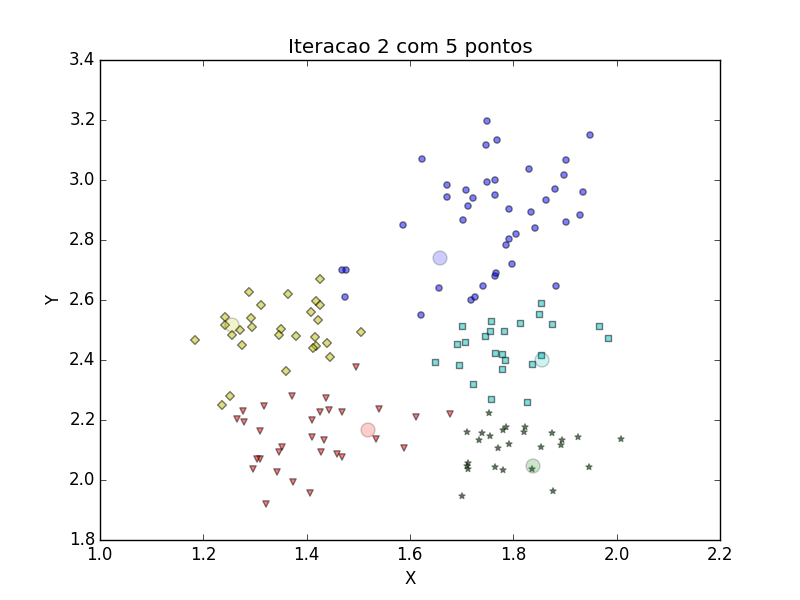
\includegraphics[width=0.4\textwidth]{depois_2.png}
    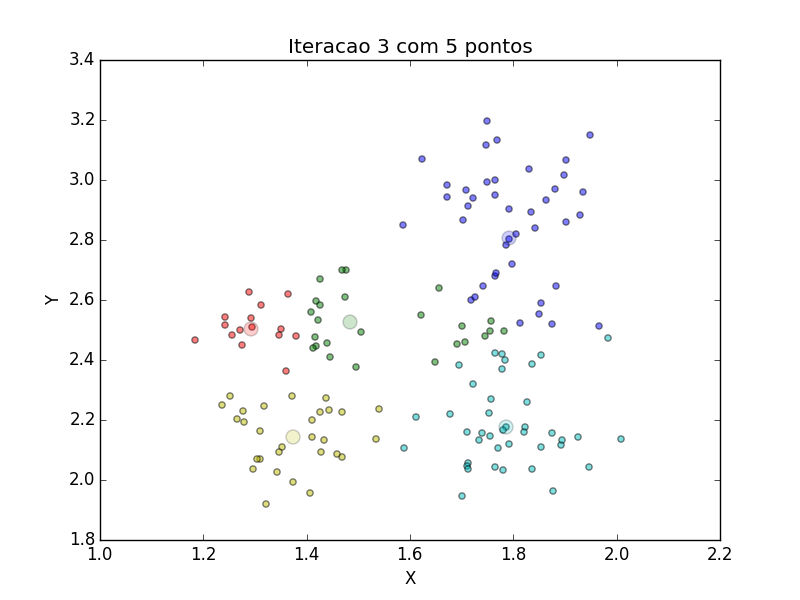
\includegraphics[width=0.4\textwidth]{depois_3.png}
    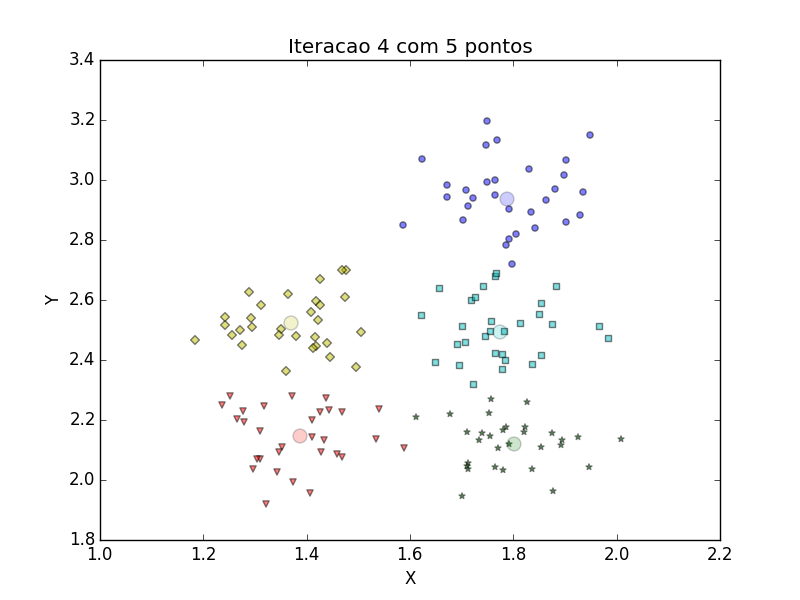
\includegraphics[width=0.4\textwidth]{depois_4.png}
    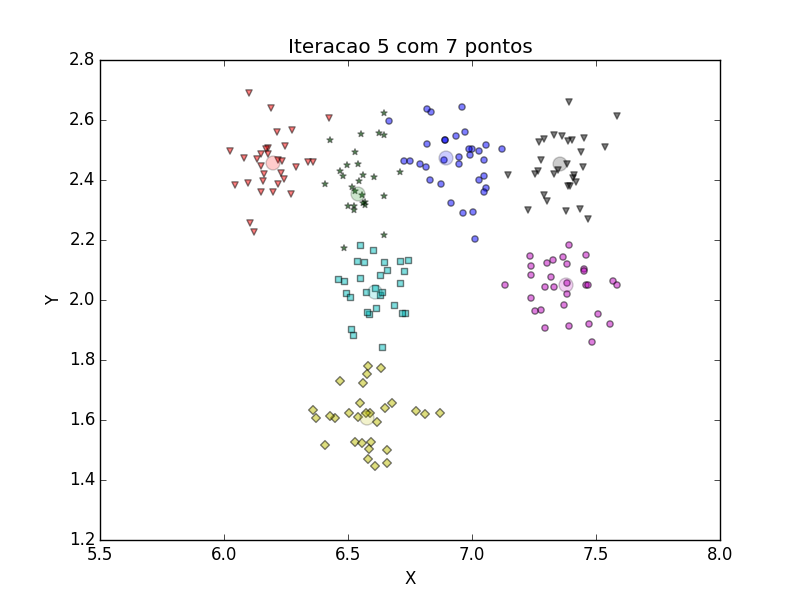
\includegraphics[width=0.4\textwidth]{depois_5.png} 
    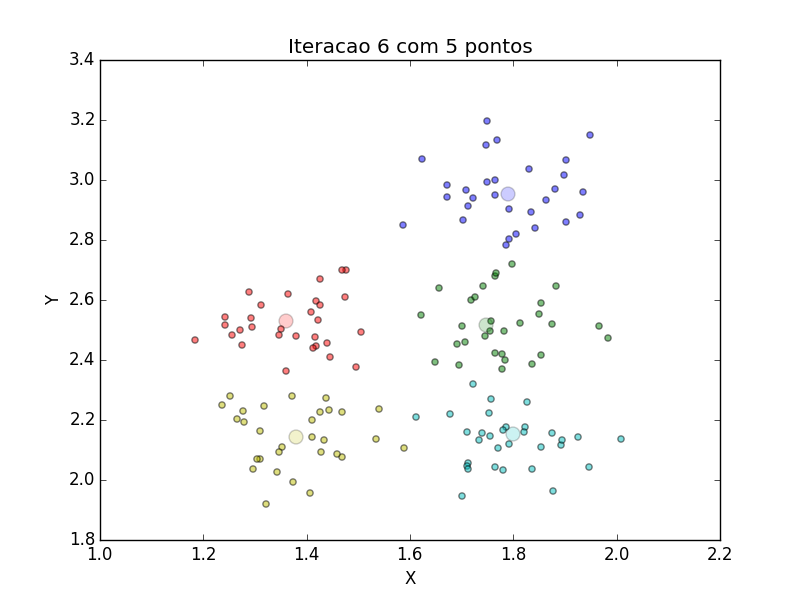
\includegraphics[width=0.4\textwidth]{depois_6.png}    
    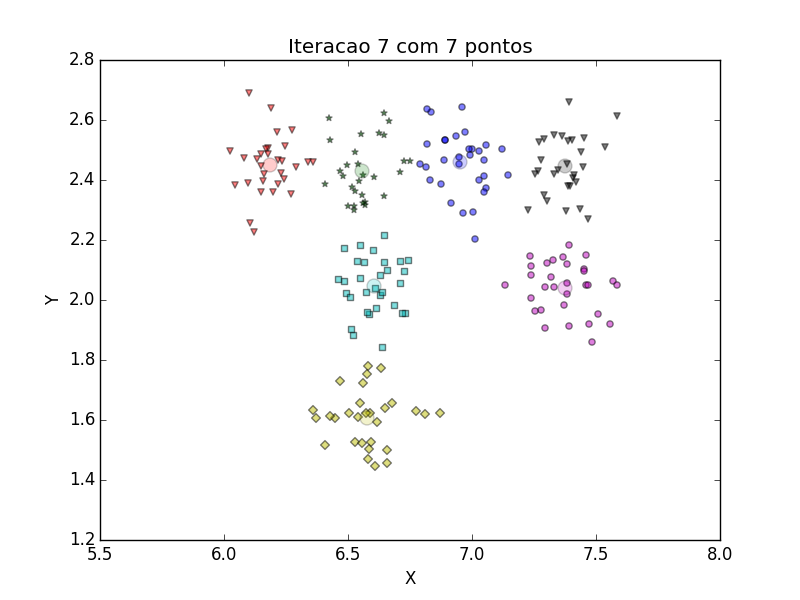
\includegraphics[width=0.4\textwidth]{depois_7.png}
    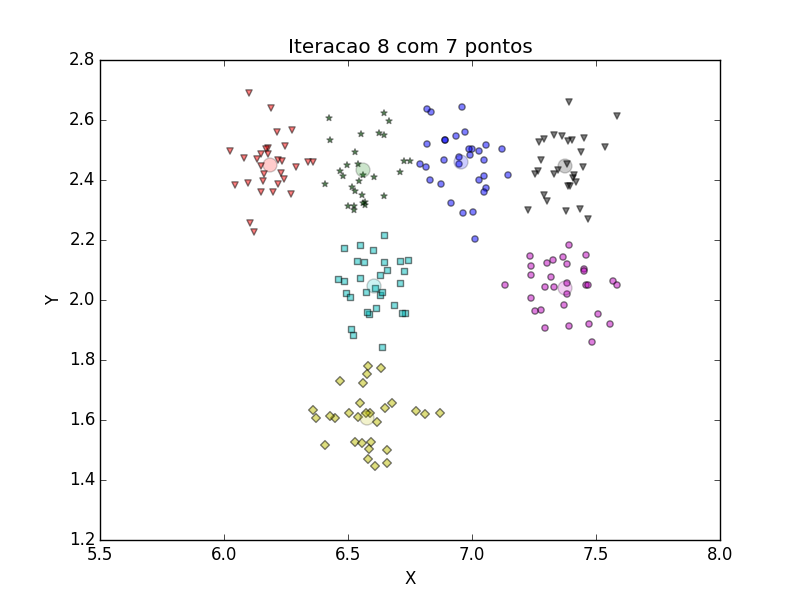
\includegraphics[width=0.4\textwidth]{depois_8.png}
\end{figure}
\end{landscape}

\newpage
\bibliography{Trabalho_IA}

\end{document}